
\chapter{Results}\label{chap:4}
% \section{Prototyping/Evaluating the System}
% 5-7 pages
% \lipsum[1]\todo{TODO}


    
This chapter will provide an overview of the achieved results, the determined baselines, the setup of the experiments, the nature of the environment and the experiment process to solve the posed research question. 
This chapter also adapts the structure for machine learning algorithms proposed by \textcite{luckert2016using}.
%  the pipeline deployment details,  collection and labelling steps, the neural network implementation and training. Finally, the pose estimation algorithms and the pipeline are evaluated.
Section \ref{chap:4:setup} illustrates the environment and sensors setup, 
section \ref{chap:4:behaviors} describes the exploration and voxel-curious behaviors setup, 
% section \ref{chap:4:train_data} explains the data collection and neural network training, 
% section \ref{chap:4:\ref{chap:4:training}} detailing the training , 
and section \ref{chap:4:results} presents the experiment results. The following questions will be answered thoroughly:
\begin{itemize}
    \item How were the experiments set up?
    % \item What was the cloud deployment setup for the solution?
    \item How many episodes, metrics, etc., were ran and collected for training, testing and optimizing the algorithms?
    % \item Which tools were used to acquire the metrics, create the data and perform the experiments?
    \item Which algorithm parameters were the most influential?
    % \item Which algorithm optimizations were done?
    \item What were the achieved results on each experiment?
    \item What was the setup of the best performing algorithm?
    % \item Which algorithm optimizations were done?
\end{itemize}

\section{Environment and Vision Setup}\label{chap:4:setup}

% As proof of concept for the project the test environment that was set up consisted of an artificial cow at the ZHAW and a robotic arm as shown by Figure \ref{fig:cow_setup}. The hardware setup for such an environment consisted of the following:


To carry out the experiments, a set of learning environments were required to train, collect metrics and test the different agent behaviors. These behaviors derivated as a result of different observations, hyperparameters, policies and reward signals. The established 3D environment is illustrated in Figure \ref{fig:unity-island}, with the respective exploration boundaries that limit the exploration space for the agent.

\begin{figure}[!ht]
    \centering
    \subfigure{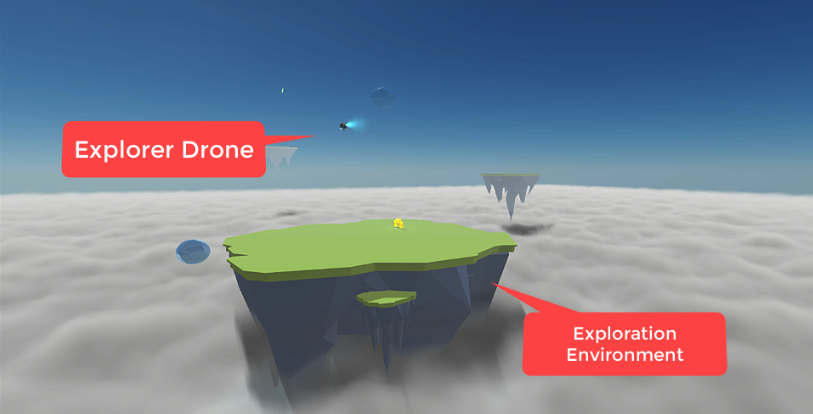
\includegraphics[width=0.49\textwidth]{images/unity-chapter4-intro.png}} 
    \subfigure{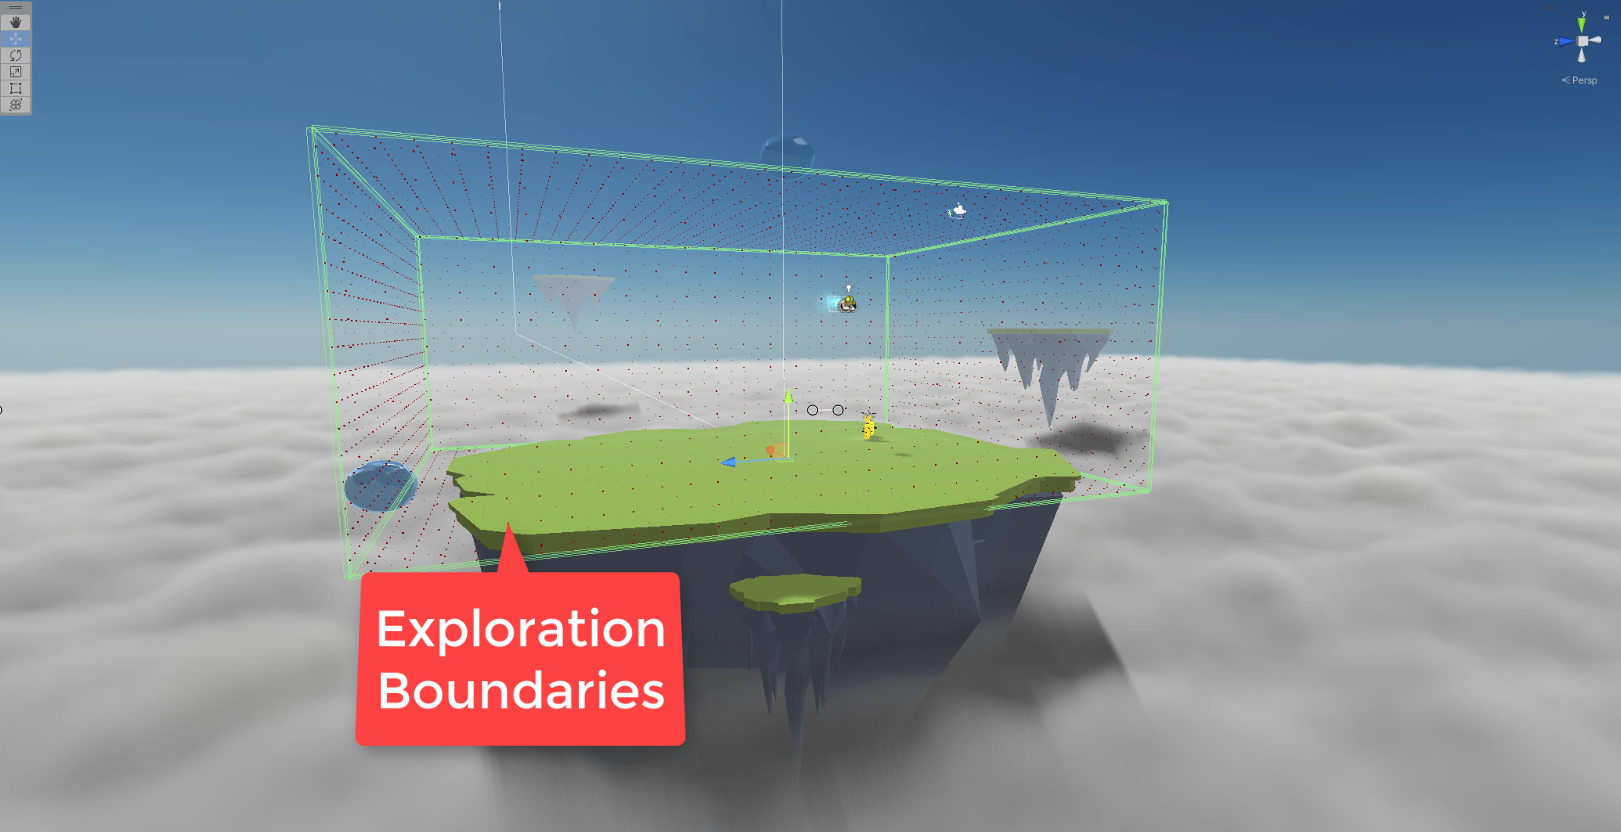
\includegraphics[width=0.49\textwidth]{images/unity-environments-training-boundaries.png}} 
    \caption{Training 3D environment in Unity 3D with explorer drone (left). Exploration boundaries of training environment to delimit evaluation zone (right). Created using 3D models from \cite{unity-asset-store}.}
    \label{fig:unity-island}
\end{figure}

As claimed by [ref], many exploration approaches shoot themselves in the foot by using methods that rely on heavy data structures in the form of point clouds, meshes, etc., which limits area they can explore. Other methods do not consider the efficiency problem at all and are short-sighted to scenarios where the goal is a couple steps ahead of the agent's starting point. We therefore compare the performance between a \textit{small} environment of 20 $m^2$ and a \textit{big} environment of 100 $m^2$ to interpret this claim. Figure \ref{fig:unity-islands-bigsmall} shows the two variants of the established 3D environment, where the big environment also includes obstacles for the agent to navigate around.


\begin{figure}[!ht]
    \centering
    \subfigure{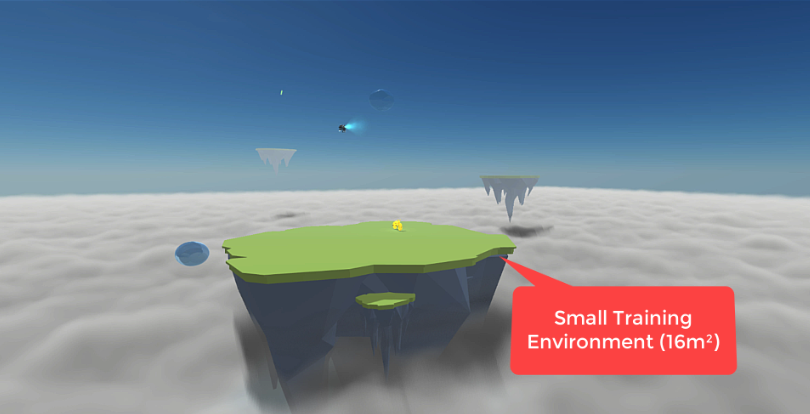
\includegraphics[width=0.49\textwidth]{images/unity-chapter4-small.png}} 
    \subfigure{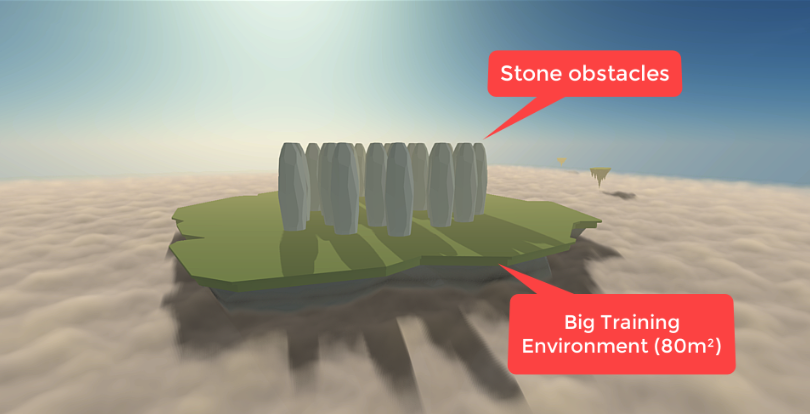
\includegraphics[width=0.49\textwidth]{images/unity-chapter4-big.png}} 
    \caption{Sample 3D assets for scenario proposals. Taken from \cite{unity-asset-store}.}
    \label{fig:unity-islands-bigsmall}
\end{figure}

Consequently, after the definition and setup of the environment, the next step is the setup of the vision system. As described in more detail in the previous chapter, the approach to perception was to use the grid sensors from \cite{github-unity-mlagents-toolkit, github-mbaske-gridsensor}. These grid sensors create a mesh of ray casts that mimic the output of a normal depth camera to interpret an abstracted view that takes the form of simplified, voxelized view of the environment. As also mentioned in the previous chapter, their output is then fed through a visual encoder that uses convolutional neural networks to transform this visual input for the agent. 

Figure \ref{fig:unity-island-gridsensors} visualizes the range of the two grid sensors used in the agent and the voxelized view they produce. One grid sensor is used to visualize elements in a panoramic fashion within a radius of 16 meters, where elements of three types are detected: boundaries, obstacles and collectibles, A second and smaller grid sensor with a diameter of 6 meters acts as the scanner in the voxel-exploration task: this grid sensor mimics a "scanneable" area and has a fail-rate of 20\% to provide the agent from an imperfect scanning behavior. Voxels that fall into this grid sensor's area are marked as scanned and accumulated by a counter to reward the agent at timestep \textit{t}. 

\begin{figure}[!ht]
    \centering
    \subfigure{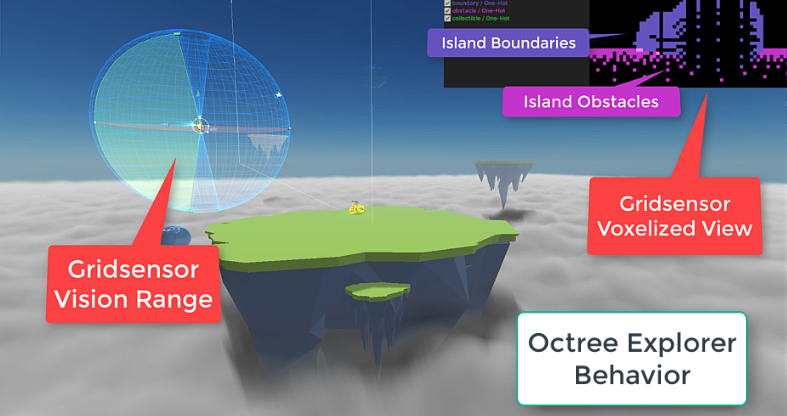
\includegraphics[width=0.49\textwidth]{images/unity-environments-training-gridsensor-single-octree.png}}
    \subfigure{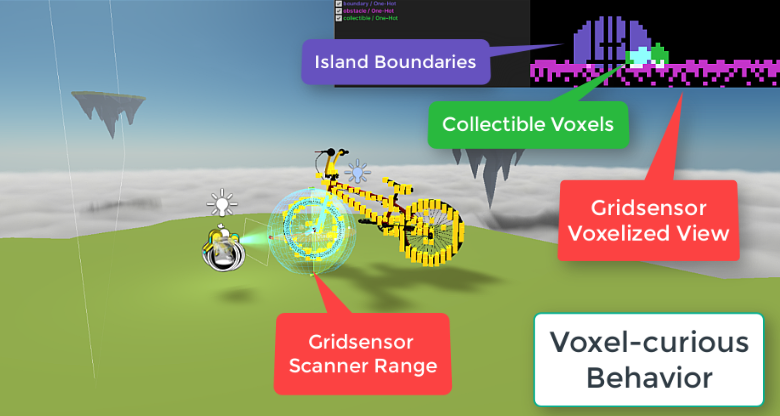
\includegraphics[width=0.49\textwidth]{images/unity-environments-training-gridsensor-single-voxel.png}} 
    \caption{Integrated grid sensor used for the agent to perceive objects, boundaries and collectibles (left). Grid sensor used by the agent as a voxel-scanner (right). Voxelized-view perceived through the grid sensors is also shown.}
    \label{fig:unity-island-gridsensors}
\end{figure}

\section{Behaviors Setup}\label{chap:4:behaviors}

The setup of the agent behaviors for the exploration of octrees and voxels is comprised by the set of observations and rewards provided to motivate a certain policy. The octree exploration policy was motivated by the approach presented by \textcite{chen2019learning}, where each discovered node in the octree provides a certain reward to the agent. To analyze the behavior of different octree setups,  diverse experiments were run with varying from nodes of 4 $m^3$ to 16 $m^3$. Therefore, the rewarding styles for octree exploration policies vary according to the size of the octree nodes the agent can discover. The diverse variants of these octree setups are presented in Table \ref{}. Table \ref{appendix:baselines_rewards} presents a complete view on the different variants trained. 

A second branch of variants of this approach take into account something called \textit{pigeon observations}. These observations take inspiration of the physiology used by pigeons to orient themselves in their environment, memorize routes and keep a biological compass. They consist of two vectors: one towards a geographical north and one towards a sun placed on top of the training island. 

Finally, following the example given by \textcite{chaplot2020semantic}, we analyze the performance of a "blind" octree variant that is curious for new states following the approach proposed by  \textcite{pathak2017curiosity} and then compare it to the octree methods that follow \textcite{chen2019learning}'s approach. Moreover, as motivated by \textcite{github-unity-mlagents-toolkit}, we go one step further and integrate \textcite{pathak2017curiosity}'s parameters into the agent's model to construct our proposed explorer drone, which takes into account all three: 1) octree observations, 2) pigeon observations and 3) pathak's curiosity for new states.


Similarly, the voxel exploration policy was motivated by a rewards-per-voxel fashion, where the diverse policies vary according to the reward per voxel, ranging from a 25\% reward per voxel to a 100\% reward per voxel. Additionally, other variants were taken to propose a \textit{normalized voxel reward} where the voxel reward has a ceiling given by $ R^{VOX} = \frac{voxels\_scanned}{2 + voxels\_scanned} $.

\begin{figure}[!ht]
    \centering
    \subfigure{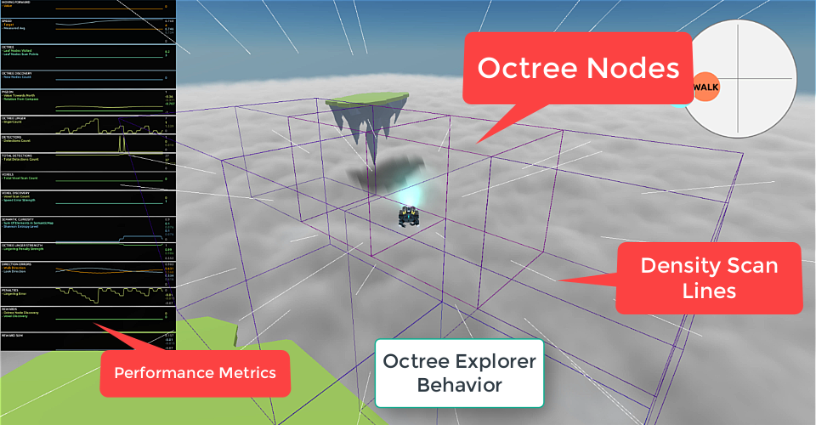
\includegraphics[width=0.49\textwidth]{images/unity-environments-training-behavior-octree2.png}} 
    \subfigure{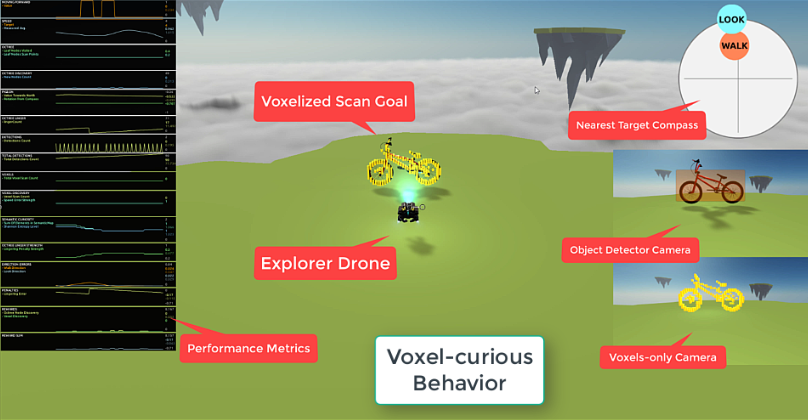
\includegraphics[width=0.49\textwidth]{images/unity-environments-training-behavior-voxel.png}} 
    \caption{Sample 3D assets for scenario proposals. Taken from \cite{unity-asset-store}.}
    \label{fig:unity-my-3d-envs}
\end{figure}

\section{Results}\label{chap:4:results}
This section presents the results of the experiments. Section \ref{chap:4:results-RQ2} deals with the results concerning the exploration of objects and \ref{chap:4:results-RQ1} deals with the results concerning the exploration of unknown spaces using octrees. Each subsection will present the best results obtained on the exploration policy variants and a brief description of the most representative details of each variant.

% • How can an embodied agent increase the overall certainty about an object’s characteristics, i.e., how
% can trajectories around objects of interest be generated to reduce the uncertainty about such objects?
% • How can these objects be found in large and unknown environments by the same agent

\subsection{Research Question 1}\label{chap:4:results-RQ1}

The first research question focuses on the reduction of uncertainty about objects, which we have posed as a voxel-curiosity task. Below, the best results for each voxel-curious variant are be presented. Detailed information about each run can be found in Appendix \ref{appendix:baselines}.

Each run was trained for 30 million timesteps using PPO and variations of the hyperparameters presented in \ref{appendix:ppo-trainer}. The training environment provided the agent 6 goals per episode situated at a distance of 5-50 meters away from the origin. In contrast, the testing environment contained a single goal located between 30 to 50 meters away from the origin. This sparse-reward testing environment evaluates the actual explorative capabilities of an agent.

A brief overview of the aggregated results is shown below in Table \ref{tab:RQ1-results}, which also shows the general performance of the algorithms for the voxel scanning task. A deeper dive into this behavior is taken in the following tables.

The run names that have a number such as \textit{run63++025} indicate that the voxel reward has a weight factor of 25\%, whereas \textit{run63++100} provides the agent a 100\% of the voxel reward. This allowed the analysis of different influences of voxel reward values and their impact on the agent's behavior. Furthermore, \textit{-constrained} indicates that the training environment manager will not reset the episode if the agent hits a boundary wall. For further information on the run names, please refer to Table \ref{appendix:baselines_rewards}.

\newpage

\begin{longtable}{|l|c|c|c|}                            \hline
% \multicolumn{3}{|l|}{\textbf{Voxel-Curiosity}}              \\\hline
\thead{Method}            
& \thead{Episode Length}                
& \thead{Average Total Objects Scanned}  
& \thead{Standard Deviation}            \\ \hline
run61-voxel	&	100	\%	&	0.34	&	0.10	\\ \hline
run61-voxel-constrained	&	100	\%	&	0.33	&	0.11	\\ \hline
run63++025	&	89	\%	&	1.56	&	0.24	\\ \hline
run63++050	&	94	\%	&	1.05	&	0.20	\\ \hline
run63++075	&	71	\%	&	0.96	&	0.17	\\ \hline
run63++100	&	99	\%	&	0.77	&	0.17	\\ \hline
run63++100-nospeed	&	97	\%	&	1.52	&	0.20	\\ \hline
run63++100-nospeed-nolinger	&	98	\%	&	1.73	&	0.21	\\ \hline
run63-normalized	&	97	\%	&	0.40	&	0.22	\\ \hline


\caption{Overview of the best object-focused runs with respect to the \textit{Total Objects Scanned} metric}. \label{tab:RQ1-results}
\end{longtable}

Table \ref{tab:results-RQ1-walkLook} shows the results for the total of voxels scanned and also their performance measured by the amount of \textit{total detections}, the \textit{walk error} and the \textit{look error}. These two errors represent the directional error to the nearest target for the agent. 

\begin{longtable}{|l|c|c|c|}                            \hline
% \multicolumn{3}{|l|}{\textbf{Walk Error}}              \\\hline
\thead{Method}            
& \thead{Total Detections Count} 
& \thead{Walk Error} 
& \thead{Look Error}   \\ \hline
run61-voxel	&	452437.65	&	0.46	&	0.45	\\ \hline
run61-voxel-constrained	&	350545.99	&	0.47	&	0.47	\\ \hline
run63++025	&	426601.17	&	0.46	&	0.37	\\ \hline
run63++050	&	426814.30	&	0.48	&	0.47	\\ \hline
run63++075	&	377998.19	&	0.47	&	0.46	\\ \hline
run63++100	&	360373.23	&	0.47	&	0.44	\\ \hline
run63++100-nospeed	&	315159.74	&	0.46	&	0.41	\\ \hline
run63++100-nospeed-nolinger	&	425433.05	&	0.47	&	0.41	\\ \hline
run63-normalized	&	\textbf{610597.65}	&	0.48	&	0.42	\\ \hline
\caption{Overview of the best runs for the object exploration task, with respect to the \textit{Walk Error} and \textit{Look Error} metrics}.
\label{tab:results-RQ1-walkLook}
\end{longtable}

The explorative performance of the best voxel-curious methods are presented in Table \ref{tab:results-RQ1-explorative-performance}, which is given by metrics such as the amount of octree scan points, the leaf nodes visited and the lingering behavior.

\begin{longtable}{|l|c|c|c|c|}                            \hline
% \multicolumn{3}{|l|}{\textbf{Voxel-Curiosity}}              \\\hline
\thead{Method}            
& \thead{Octree \\ Scan Points} 
& \thead{Octree \\ Leaf Nodes Visited} 
& \thead{Lingering \\ Penalty Count}  
& \thead{Lingering \\ Penalty Strength} 
\\ \hline
% run61-voxel	&	36.15	&	10.07	&	24.67	&	0.95	\\ \hline
% run61-voxel-constrained	&	42.58	&	14.06	&	19.20	&	0.96	\\ \hline
% run63++025	&	\textbf{131.40}	&	\textbf{40.18}	&	\textbf{31.10}	&	0.95	        \\ \hline
% run63++050	&	83.43	&	28.41	                &	24.20	&   0.95	        \\ \hline
% run63++075	&	90.33	&	29.63	                &	11.27	&   0.96	        \\ \hline
% run63++100-nospeed-nolinger	&	119.59	&	36.28	&	\textbf{30.26}	&	0.95	        \\ \hline
% run63++100-nospeed	&	\textbf{126.73}	&	36.67	&	16.15	&	0.96	        \\ \hline
% run63++100	&	87.74	&	29.11	                &	\textbf{25.61}   &   0.96	        \\ \hline
% run63-normalized	&	97.68	&	31.45	        &	9.92    &   0.93	        \\ \hline
run61-voxel	&	36.15		&	0.3	\%	&	24.67	&	0.95	\\ \hline
run61-voxel-constrained	&	0.00		&	0.4	\%	&	19.20	&	0.96	\\ \hline
run63++025	&	131.40		&	1.0	\%	&	31.10	&	0.95	\\ \hline
run63++050	&	83.43		&	0.7	\%	&	24.20	&	0.95	\\ \hline
run63++075	&	90.33		&	0.7	\%	&	11.27	&	0.96	\\ \hline
run63++100	&	87.74		&	0.7	\%	&	25.61	&	0.96	\\ \hline
run63++100-nospeed	&	126.73		&	0.9	\%	&	16.15	&	0.96	\\ \hline
run63++100-nospeed-nolinger	&	119.59		&	0.9	\%	&	30.26	&	0.95	\\ \hline
run63-normalized	&	97.68		&	0.8	\%	&	9.92	&	0.93	\\ \hline


\caption{Overview of the best runs for the object exploration task, with respect to the \textit{Octree Scan Points}, \textit{Octree Leaf Nodes Visited}, \textit{Lingering Penalty Strength} and \textit{Lingering Penalty Count} metrics}. \label{tab:results-RQ1-explorative-performance}
\end{longtable}


% \begin{longtable}{|l|c|c|c|c|}                            \hline
% % \multicolumn{3}{|l|}{\textbf{Voxel-Curiosity}}              \\\hline
% \textbf{Method}            
% & \thead{Speed Error}
% & \thead{Voxel Scanned} 
% & \thead{Octree Lingering \\ Count}
% & \thead{Detections Total \\ Count}   \\ \hline
% run64       & 260k      & No       & a & b                  \\ \hline
% \caption{Overview of the best runs for the object exploration task, with respect to the \textit{Octree Discovery Reward} metric}. \label{tab:RQ1-results}
% \end{longtable}

\subsection{Research Question 2}\label{chap:4:results-RQ2}

This section deals with the results related to question 2, which focuses on the exploration of the 3D space in a given environment using octrees. The 160$m^2$ environment consists of around 8000, 800 and 200 nodes when segmented in octants of 4$m^3$, 8$m^3$ and 16$m^3$, respectively. The following Table \ref{tab:RQ2-results} summarizes the best models for the explorative task using the octree discovery reward.

% The presented numbers are the result of 500000 optimizations 
\begin{longtable}{|l|c|c|c|}                            \hline
% \multicolumn{3}{|l|}{\textbf{Voxel-Curiosity}}              \\\hline
\textbf{Method}            
& \thead{Episode Length}                
& \thead{Octree Discovery Reward}                
& \thead{Standard Deviation}            \\ \hline
% run61-explore	&	95	\%	&	0.89	&	0.07	\\ \hline
run61-explore-constrained	&	100	\%	&	0.93	&	0.03	\\ \hline
run62-4	&	97	\%	&	0.83	&	0.03	\\ \hline
run62-4-pigeon	&	19	\%	&	0.22	&	0.05	\\ \hline
run62-4-pigeon-pathak	&	25	\%	&	0.21	&	0.06	\\ \hline
run62-8	&	49	\%	&	0.18	&	0.05	\\ \hline
run62-8-pathak	&	63	\%	&	0.15	&	0.02	\\ \hline
run62-16	&	4	\%	&	0.07	&	0.00	\\ \hline
run62-16-constrained	&	100	\%	&	0.01	&	0.00	\\ \hline
run62-16-constrained-pigeon	&	100	\%	&	0.03	&	0.01	\\ \hline
run62-16-constrained-pigeon-pathak	&	100	\%	&	0.01	&	0.00	\\ \hline
run62-16-pathak	&	4	\%	&	0.07	&	0.00	\\ \hline

\caption{Overview of the best environment-exploration focused runs with respect to the \textit{Octree Discovery Reward} metric}. \label{tab:RQ2-results}
\end{longtable}

The contrast in explorative performance for the best octree exploration methods and the best voxel-curious methods is presented below in Table \ref{tab:RQ2-results-comparative-voxeloctree}. This contrast is based on the number of scan points, the number of leaf nodes and the lingering behavior. 

\begin{longtable}{|l|c|c|c|}                            \hline
% \multicolumn{3}{|l|}{\textbf{Voxel-Curiosity}}              \\\hline
\thead{Method}            
& \thead{Octree Scan \\ Points Found}
& \thead{Octree \\ Lingering Count}
& \thead{Octree Leaf  \\ Nodes Visited}   \\ \hline
% run61-explore	        &	1\%	&	3.14	&	1\%	\\ \hline
% run61-explore-constrained	        &	2\%	&	3.11	&	1\%	\\ \hline
% run62-4     	&	1\%	&	3.11	&	1\%	\\ \hline
% run62-4-pigeon	        &	0\%	&	6.94	&	0\%	\\ \hline
% run62-4-pigeon-pathak	&	1\%	&	8.39	&	0\%	\\ \hline
% run62-8     	&	5\%	&	7.05	&	3\%	\\ \hline
% run62-8-pathak      	&	5\%	&	7.20	&	3\%	\\ \hline
% run62-16	        &	6\%	&	10.07	&	1\%	\\ \hline
% run62-16-constrained	        &	\textbf{24\%}	&	4.99	&	\textbf{11\%}	\\ \hline
% run62-16-constrained-pigeon	        &	\textbf{21\%}	&	3.68	&	\textbf{17\%}	\\ \hline
% run62-16-constrained-pigeon-pathak	&	15\%	&	5.66	&	5\%	\\ \hline
% run62-16-pathak	        &	6\%	&	9.91	&	1\%	\\ \hline
% run61-explore	&	3.0	\%	&	3.14	&	2.3	\%	\\ \hline
run61-explore-constrained	&	3.5	\%	&	3.11	&	2.4	\%	\\ \hline
run62-4	&	2.3	\%	&	3.11	&	2.3	\%	\\ \hline
run62-4-pigeon	&	0.7	\%	&	6.94	&	0.3	\%	\\ \hline
run62-4-pigeon-pathak	&	1.0	\%	&	8.39	&	0.3	\%	\\ \hline
run62-8	&	12.2	\%	&	7.05	&	6.5	\%	\\ \hline
run62-8-pathak	&	11.9	\%	&	7.20	&	7.3	\%	\\ \hline
run62-16	&	7.5	\%	&	10.07	&	1.7	\%	\\ \hline
run62-16-constrained	&	30.2	\%	&	4.99	&	13.5	\%	\\ \hline
run62-16-constrained-pigeon	&	26.4	\%	&	3.68	&	21.5	\%	\\ \hline
run62-16-constrained-pigeon-pathak	&	19.0	\%	&	5.66	&	5.9	\%	\\ \hline
run62-16-pathak	&	8.0	\%	&	9.91	&	1.7	\%	\\ \hline
\caption{Overview of the best runs for the object exploration task, with respect to the \textit{Octree Scan Points Found}, \textit{Octree Lingering Count} and \textit{Octree Leaf Nodes Visited} metrics}. \label{tab:RQ2-results-comparative-voxeloctree}
\end{longtable}


\subsection{Mixed-Focus Agents}
This sections presents the variant of agents that have both knowledge of the environment and voxels. Information about the environment can be present in the form of octree nodes, lingering feedback and \textit{pigeon observations}. Table \ref{tab:results-mixed-agents} displays the results for this run.

\begin{longtable}{|l|c|c|c|c|c|c|c|}                            \hline
% \multicolumn{3}{|l|}{\textbf{Voxel-Curiosity}}              \\\hline
\thead{Method}            
& \thead{Total Objects \\ Scanned} 
& \thead{Look \\ Direction}
& \thead{Octree \\Reward}
& \thead{Octree Leaf \\ Nodes Visited}
& \thead{Detections \\Total Count}
& \thead{Semantic \\ Curiosity}
& \thead{Shannon \\ Entropy}             \\ \hline
run64       & 260k      & No       & a & b &  a & b    & b                 \\ \hline
run64       & 260k      & No       & a & b &  a & b    & b                 \\ \hline
run64       & 260k      & No       & a & b &  a & b    & b                 \\ \hline
run64       & 260k      & No       & a & b &  a & b    & b                 \\ \hline
run64       & 260k      & No       & a & b  & a & b    & b                  \\ \hline
run64       & 260k      & No       & a & b  & a & b    & b                  \\ \hline
run64       & 260k      & No       & a & b  & a & b    & b                  \\ \hline
run64       & 260k      & No       & a & b  & a & b    & b                  \\ \hline
run64       & 260k      & No       & a & b  & a & b    & b                  \\ \hline
\caption{Overview of the best runs for the object exploration task, with respect to the \textit{Total Objects Scanned}, \textit{Look Direction}, \textit{Octree Reward}, \textbf{Octree Leaf Nodes Visited}, \textit{Detections Total Count}, \textbf{Semantic Curiosity} and \textbf{Shannon Entropy} metrics}. \label{tab:results-mixed-agents}
\end{longtable}


\subsection{Evaluation Framework}
This section presents the performance of the methods that serve as baselines to compare the performance of our proposed method. These baselines were also trained under different parameter configurations to reach the best performant one, as displayed in Table \ref{tab:results-evaluation-framework} with the metrics collected and the baselines used to evaluate our method 
The baselines were setup using

\begin{longtable}{|l|c|c|c|c|c|c|c|}                            \hline
% \multicolumn{3}{|l|}{\textbf{Voxel-Curiosity}}              \\\hline
\thead{Method}            
& \thead{Total Objects \\ Scanned} 
& \thead{Look \\ Direction}
& \thead{Octree \\Reward}
& \thead{Octree Leaf \\ Nodes Visited}
& \thead{Detections \\Total Count}
& \thead{Semantic \\ Curiosity}
& \thead{Shannon \\ Entropy}             \\ \hline
run64       & 260k      & No       & a & b &  a & b    & b                 \\ \hline
run64       & 260k      & No       & a & b &  a & b    & b                 \\ \hline
run64       & 260k      & No       & a & b &  a & b    & b                 \\ \hline
run64       & 260k      & No       & a & b &  a & b    & b                 \\ \hline
run64       & 260k      & No       & a & b  & a & b    & b                  \\ \hline
run64       & 260k      & No       & a & b  & a & b    & b                  \\ \hline
run64       & 260k      & No       & a & b  & a & b    & b                  \\ \hline
run64       & 260k      & No       & a & b  & a & b    & b                  \\ \hline
run64       & 260k      & No       & a & b  & a & b    & b                  \\ \hline
run64       & 260k      & No       & a & b  & a & b    & b                  \\ \hline
\caption{Overview of the best runs for the object exploration task, with respect to the \textit{Total Objects Scanned}, \textit{Look Direction}, \textit{Octree Reward}, \textbf{Octree Leaf Nodes Visited}, \textit{Detections Total Count}, \textbf{Semantic Curiosity} and \textbf{Shannon Entropy} metrics}. \label{tab:results-evaluation-framework}
\end{longtable}


\subsection{Small Environment Results}\label{chap-4:small-env-results}
This section presents the best performances for the voxel exploration task and the octree exploration task. The corresponding results for the big environment were presented in Sections \ref{chap:4:results-RQ1} and \ref{chap:4:results-RQ2} respectively. As mentioned before, the small environment has an area of 16 $m^2$ and the big environment has an area of 80 $m^2$. 
The only difference is that the agent's grid sensor for the small environment has a smaller range with a radius of 8 meters.

Table \ref{tab:results-small-env-voxel} displays the best runs for the voxel-curious behaviors in the small environment.

\begin{longtable}{|l|c|c|c|c|c|c|c|}                            \hline
% \multicolumn{3}{|l|}{\textbf{Voxel-Curiosity}}              \\\hline
\thead{Method}            
& \thead{Average Total Objects Scanned}  
& \thead{Standard Deviation}            \\ \hline

run61	&	0.00	&	0.00	\\ \hline
run62	&	0.00	&	0.00	\\ \hline
run63	&	3.03	&	1.84	\\ \hline
run63++025	&	4.76	&	\textbf{2.37}	\\ \hline
run63++050	&	1.49	&	0.47	\\ \hline
run63++075	&	2.62	&	0.88	\\ \hline
run63++100	&	\textbf{9.42}	&	0.39	\\ \hline
run64	&	0.00	&	0.00	\\ \hline
run65	&	0.03	&	0.01	\\ \hline
run65	&	0.01	&	0.03	\\ \hline
run65-pure	&	\textbf{8.71}	&	0.56	\\ \hline
run66	&	0.35	&	0.12	\\ \hline
run66	&	0.16	&	0.08	\\ \hline
run67	&	0.00	&	0.00	\\ \hline
run68	&	0.00	&	0.00	\\ \hline
run68++050	&	\textbf{9.19}	&	0.41	\\ \hline
run68++100	&	\textbf{9.04}	&	0.66	\\ \hline

\caption{Overview of the results for the runs in the small environment, with respect to the \textit{Total Objects Scanned} metric}.
\label{tab:results-small-env-voxel}
\end{longtable}


% \newpage
The following Table \ref{tab:results-small-env-octree} presents the runs with the best performance in the octree exploration task.
 
\begin{longtable}{|l|c|c|}                            \hline
% \multicolumn{3}{|l|}{\textbf{Voxel-Curiosity}}              \\\hline
\textbf{Method}            
& \thead{Octree Discovery Reward} 
& \thead{Standard Deviation}            \\ \hline
run61	&	0.04	&	0.00	\\ \hline
run62	&	\textbf{0.09}	&	0.00	\\ \hline
run63	&	0.04	&\textbf{	0.01}	\\ \hline
run63++025	&	0.04	&	0.00	\\ \hline
run63++050	&	0.03	&	0.00	\\ \hline
run63++075	&	0.04	&	0.00	\\ \hline
run63++100	&	0.03	&	0.00	\\ \hline
run64	&	0.00	&	0.00	\\ \hline
run65	&	0.02	&	0.00	\\ \hline
run65-pure	&	0.03	&	0.00	\\ \hline
run66	&	0.02	&	0.00	\\ \hline
run67	&	0.00	&	0.00	\\ \hline
run68	&	0.04	&	0.00	\\ \hline
run68++050	&	0.04	&	0.00	\\ \hline
run68++100	&	0.04	&	0.00	\\ \hline


\caption{Overview of the results for the runs in the small environment, with respect to the \textit{Octree Discovery Reward} metric}.
\label{tab:results-small-env-octree}
\end{longtable}

The complete results of the small environment can be found in Figure \ref{fig:results-small-env-performances}


\subsection{Panoramic Performance}
This section presents the performance performed by the panoramic grid sensor and a \textit{55 degrees} wide grid sensor. This latter, narrower, grid sensor represents ordinary cameras that have a smaller field of view \cite{2020_camera_degrees}. The following Table \ref{tab:results-panoramic} therefore compares the total objects scanned, the look direction, the octree reward and related metrics that would indicate key performance differences based on the camera system. 

\begin{longtable}{|l|c|c|c|c|c|c|c|}                            \hline
% \multicolumn{3}{|l|}{\textbf{Voxel-Curiosity}}              \\\hline
\thead{Method}            
& \thead{Total Objects \\ Scanned} 
% & \thead{Look \\ Direction}
& \thead{Octree \\Reward}
& \thead{Octree Leaf \\ Nodes Visited}
& \thead{Detections \\Total Count}
& \thead{Semantic \\ Curiosity}
& \thead{Shannon \\ Entropy}             \\ \hline
with K of voxels       & 260k      & No       & a & b &  a & b                    \\ \hline
without K of voxels       & 260k      & No       & a & b &  a & b                   \\ \hline
with K of octrees       & 260k      & No       & a & b &  a & b                    \\ \hline
without K of octrees       & 260k      & No       & a & b &  a & b                    \\ \hline
\caption{Overview of the best runs for the object exploration task, with respect to the \textit{Total Objects Scanned}, \textit{Look Direction}, \textit{Octree Reward}, \textbf{Octree Leaf Nodes Visited}, \textit{Detections Total Count}, \textbf{Semantic Curiosity} and \textbf{Shannon Entropy} metrics}. \label{tab:results-panoramic}
\end{longtable}



\subsection{PPO vs SAC}

To compare the sample efficiency of PPO and SAC, we trained the best PPO-models using SAC. The following Table \ref{tab:results-SAC} displays the peformance of such models and    of experiments to demonstrate the sample efficiency of PPO. We measure the number of episodes and the number of actions to the state transition in the environment. In addition, we analyze the training speed in our experiments.

\begin{longtable}{|l|c|c|c|c|c|c|c|}                            \hline
% \multicolumn{3}{|l|}{\textbf{Voxel-Curiosity}}              \\\hline
\thead{Method}            
& \thead{Episode Length \\ Direction}
& \thead{Total Objects \\ Scanned} 
& \thead{Octree \\Reward}
& \thead{Octree Leaf \\ Nodes Visited}
& \thead{Detections \\Total Count} \\ \hline
% & \thead{Semantic \\ Curiosity}
% & \thead{Shannon \\ Entropy}             \\ \hline
with K of voxels       & 260k      & No       & a & b &  a           \\ \hline
without K of voxels       & 260k      & No       & a & b &  a             \\ \hline
with K of octrees       & 260k      & No       & a & b &  a             \\ \hline
without K of octrees       & 260k      & No       & a & b &  a               \\ \hline
\caption{Overview of the best runs for the object exploration task, with respect to the \textit{Total Objects Scanned}, \textit{Look Direction}, \textit{Octree Reward}, \textbf{Octree Leaf Nodes Visited}, \textit{Detections Total Count}, \textbf{Semantic Curiosity} and \textbf{Shannon Entropy} metrics}. \label{tab:results-SAC}
\end{longtable}



% \subsection{Research Scenarios}
\subsection{Applicable Benchmark Scenarios} % Future

% \begin{figure}[!ht]
%     \centering
%     \subfigure{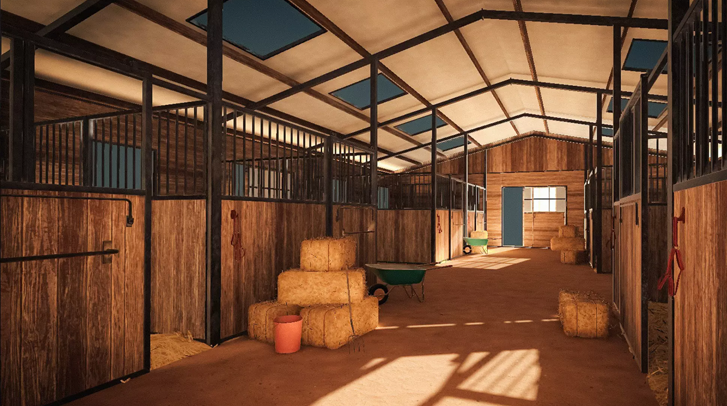
\includegraphics[width=0.32\textwidth]{images/unity-environments-stables.png}} 
%     \subfigure{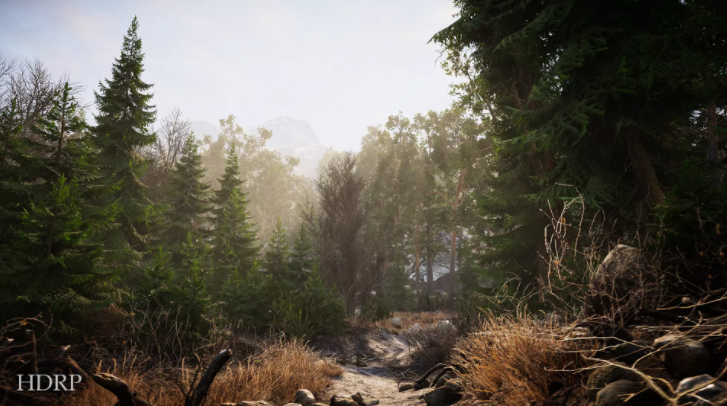
\includegraphics[width=0.32\textwidth]{images/unity-environments-forest.png}} 
%     \subfigure{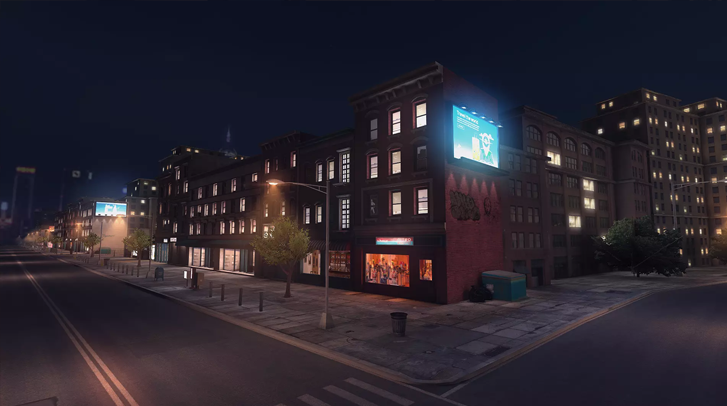
\includegraphics[width=0.32\textwidth]{images/unity-environments-city.png}}
%     \subfigure{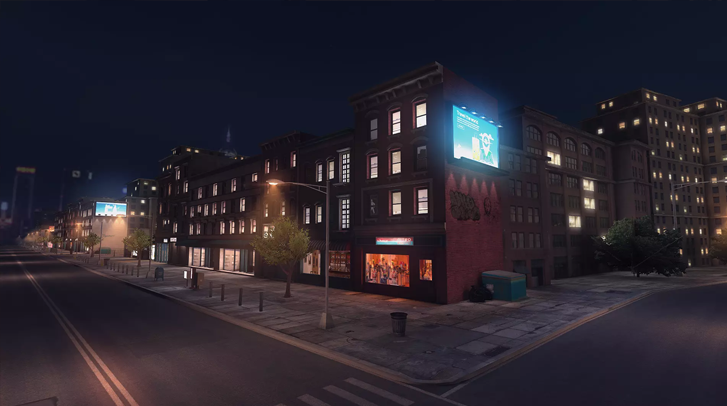
\includegraphics[width=0.32\textwidth]{images/unity-environments-city.png}}
%     \caption{Sample 3D assets for scenario proposals. Taken from \cite{unity-asset-store}.}
%     \label{fig:unity-my-3d-envs}
% \end{figure}

\begin{figure}[!ht]
    \centering
    \subfigure[Dreamscape Scenario.]{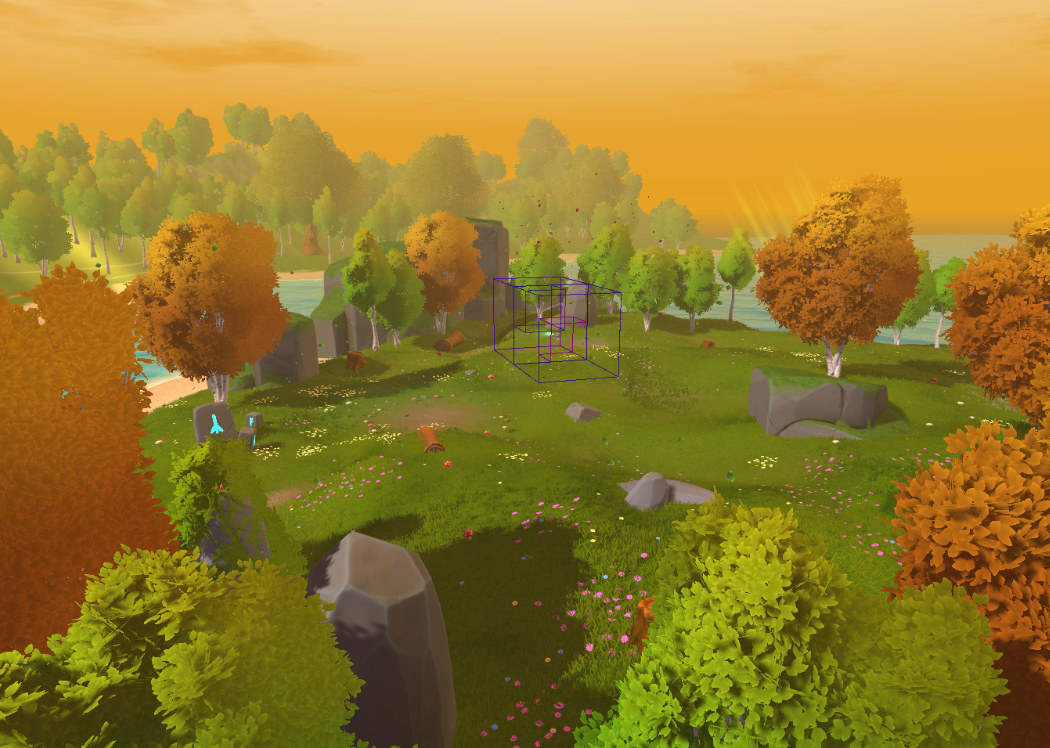
\includegraphics[width=0.245\textwidth]{images/unity-env-dreamscape.png} } 
    \subfigure[City Neighborhood.]{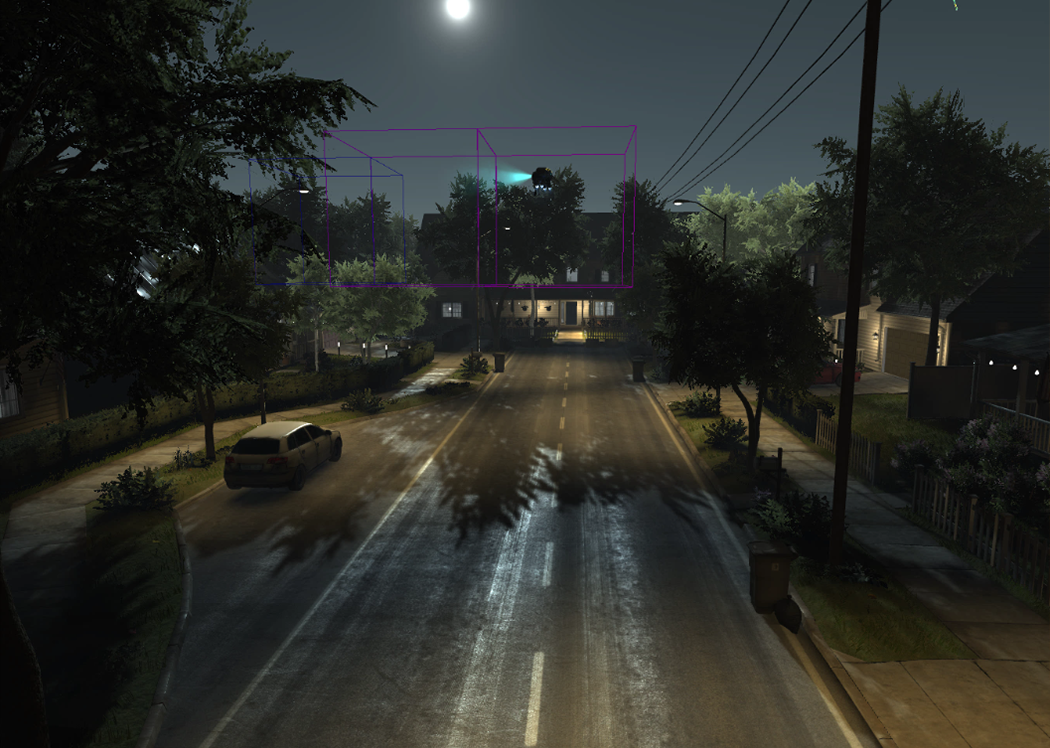
\includegraphics[width=0.245\textwidth]{images/unity-env-neighborhood.png}} 
    \subfigure[Snowy Forest.]{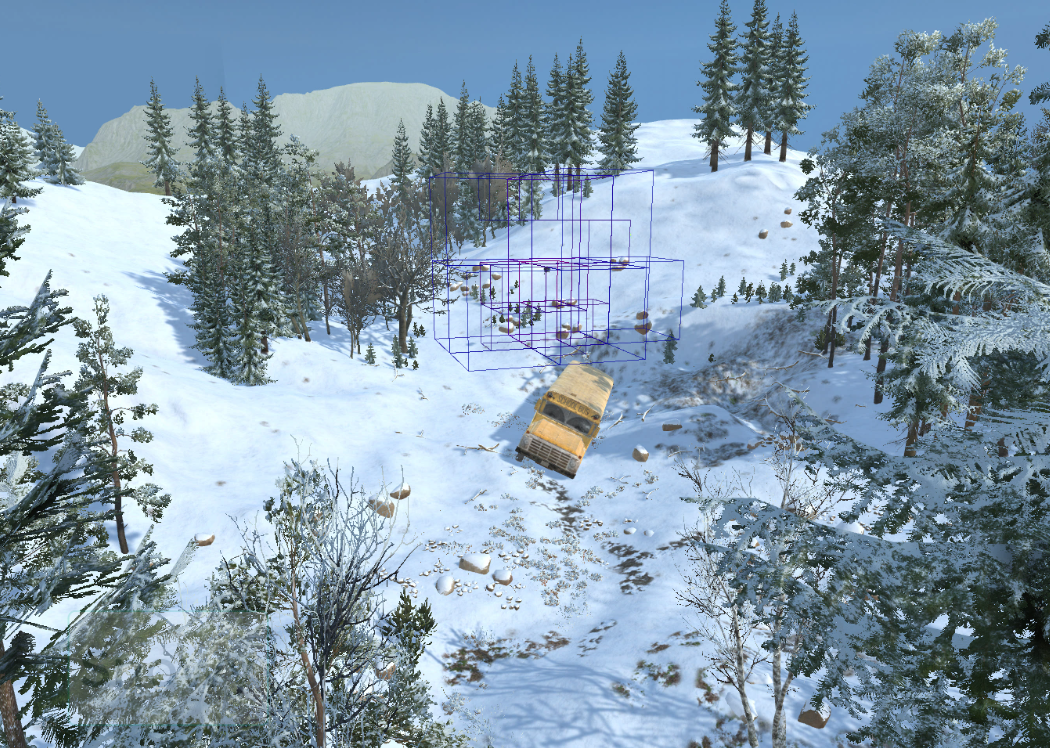
\includegraphics[width=0.245\textwidth]{images/unity-env-forest-snowy.png}}
    \subfigure[Summer Forest.]{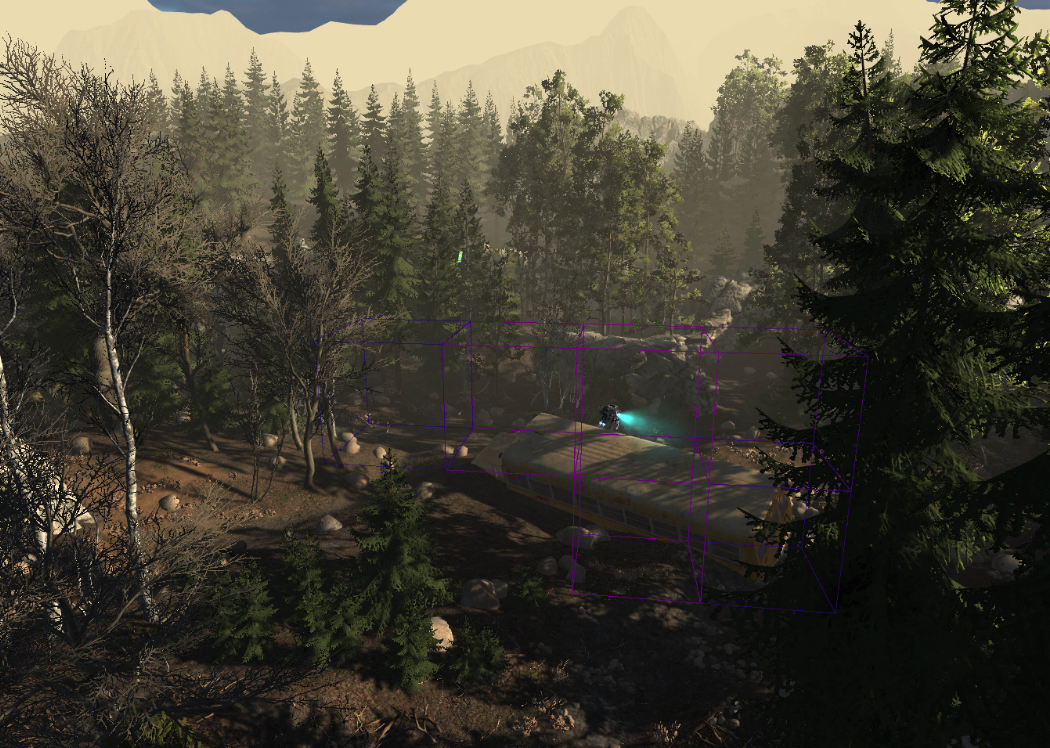
\includegraphics[width=0.245\textwidth]{images/unity-env-forest.png}}
    \caption{
        Modelled 3D scenarios to present the practical aspect of the proposed methods. 3D models subject to copyright from         
        \textcite{unity-asset-store}.
    }
    \label{fig:unity-my-3d-envs}
\end{figure}

% \begin{figure}[!ht]
%         \centering
%         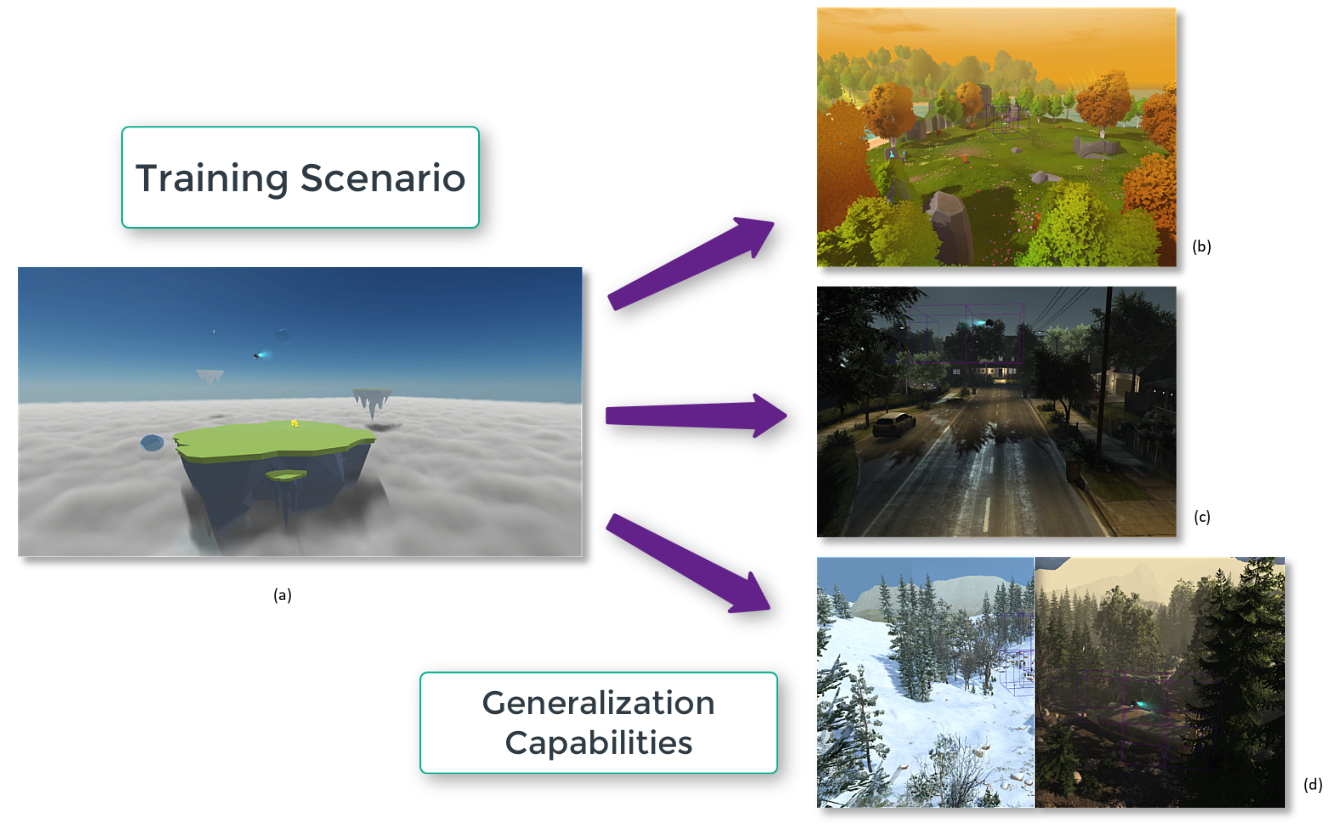
\includegraphics[width=0.6\textwidth]{images/unity-env-scenarios2.png}
%         \caption{Research Scenarios results.}
%         \label{fig:unity-simple-encoder}
% \end{figure}


Multiple 3D scenes have been collected and setup to demonstrate the applicability of our method in practical real world scenarios. Given the time constraint, deeper demonstrations of these specific use cases are out of scope.
% need to be modelled and constructed to demonstrate the applicability of the learned behavior across a variety of scenarios. 
Figure \ref{fig:unity-my-3d-envs} illustrates the training environment and different environments which were used to demonstrate the octree explorer agent's versatility to multiple environments.
\begin{itemize}
    \item \textbf{"Dreamscape".} A fantasy forest scene.
    % in reference to the milking robot scenario from our industry partner, Sutter Landtechnik GmbH (SLG).
    \item \textbf{Forest.} An open nature scene with obstacles and a bus that was drove off as part of an accident.
    \item \textbf{City Neighborhood.} A city scene where fires could be prevented with firefighter drones.
    % that presents buildings and rooms to navigate and explore.
\end{itemize}

Similarly , the voxel-curious agent showed visual agnostic performance to other voxelized objects such as bus and house, which are part of the environments below. Finally, \textit{quidditch} goalposts were also used to test knowledge transferability.


% \subsection{Cross-Scenario Performance}

% The agent showed visual agnostic performance for our agent that was trained on a voxelized bicycle and then tested on a voxelized bus and voxelized house. Moreover, an additional \textit{quidditch} scene was tested, and the agent X showed the best cross-scenario performance. Below are the metrics collected for the cross-scenario performance:

% X

\subsection{Cross-Platform Compatibility}
This section presents the results of the metrics determined to evaluate the effort of transferring the Unity ML-Agents environment to an OpenAI Gym compatible implementation. We define a compatible implementation as one that is ready to be trained and produce relevant results. The metrics are displayed in Table \ref{tab:results-cross-platform}.

\begin{longtable}{|l|c|c|}                            \hline
% \multicolumn{3}{|l|}{\textbf{Voxel-Curiosity}}              \\\hline
\textbf{Metric}            
& \thead{Value}  \\ \hline
Lines of code                                       & ~1500                          \\ \hline
Time required to transition the environment             & ~4h                           \\ \hline
Time required to integrate to WandB                     & ~20h                       \\ \hline
Time required to implement resuming of experiments       & ~40h                        \\ \hline
Time required for other features                        & ~40h                        \\ \hline
\caption{Overview of cross-platform effort measurement metrics.}.
\label{tab:results-cross-platform}
\end{longtable}



% \begin{figure}
% \includegraphics[width=1.0\linewidth]{figs/results-on-robots-tutorial/sacs-performance.pdf}
% \caption{Performance comparison of the PPO, SAC, and a vanilla RL agent.}
% \label{fig:sacs-performance}
% \end{figure}





% Table \ref{tab:test-results} provides a brief summary of the results and the general performance of the used algorithms, which are discussed afterwards in more detail.
% \newpage

% \begin{longtable}
% {@{} l c c @{}} \toprule
% \textbf{Method}                     & \textbf{Accuracy}     & \textbf{Standard Deviation}       \\ \midrule
% % PCA                                 & 97\%                  & 0.015                             \\ \midrule
% MAV                                 & \textbf{97\% }                 & \textbf{0.43}                             \\ \midrule
% DOPE                                & 0\%                  & -                             \\ \midrule
% RANSAC                              & 0\%                   & -                             \\ \bottomrule
% \caption{Statistics of tested methods.} \label{tab:test-results}                          \\
% \end{longtable}

% The following Table \ref{tab:DOPE-results} displays the results for the DOPE algorithm. DOPE uses FAT formatted data sets, which are generated using NDDS, in Unreal Engine 4. These data sets are characterized for being synthetic photorealistic images. The data set variants presented below are optimized by modifying the parameters in data set used, such as:
% % The variants used include changes in: 
% the realism degree in the materials used for the object textures, the usage of rotation in the focus object, and the usage of obstructive objects. Aditionally, all data sets include five different photorealistic scenes: beach, studio, temple, meadow and zen garden. Surprisingly none of the data sets were realistic enough to close the reality gap, which reflected in DOPE not outputting any predictions.



% \begin{longtable}{|l|c||c|}                            \hline
% \multicolumn{3}{|l|}{\textbf{Deep Object Pose}}              \\\hline
% \textbf{Dataset}            & \textbf{Size}  & \textbf{Functional}            \\ \hline
% NDDS Photorealistic (base)       & 260k      & No                             \\ \hline
% NDDS with Rotation          & 80k       & No                             \\ \hline
% NDDS Small                  & 20k       & No                             \\ \hline
% \caption{Overview of the best DOPE results for the respective dataset variations.} \label{tab:DOPE-results}
% \end{longtable}


% The results for the RANSAC algorithm are shown in Table \ref{tab:ransac-results}. The skimage implementation was used for both RANSAC and direct ORB matching. The variants presented were surprinsingly not succesful at matching X. It is suspected that RANSAC and ORB matching are not the best approach for identifying simple texture objects such as the cow teats. 
% Figure \ref{fig:ransac-results} illustrates the suspicion and the behavior of RANSAC on both the RGB and the depth images. RANSAC was tested by varying the ORB number of keypoints, the ORB threshold and RANSAC's residual threshold as well as adding a denoising step.  


% \begin{longtable}{|c|c|c|c||c|}                            \hline
% \multicolumn{5}{|l|}{\textbf{RANSAC / ORB Matching}}              \\\hline
% \textbf{ORB \#keypoints} & \textbf{ORB threshold} & \textbf{Residual Threshold} & \textbf{Denoising}       & \textbf{Functional}      \\ \hline
%         20      & 0.08      & N/A (ORB matching)       & No     &  No               \\ \hline
%         200     & 0.08      & N/A (ORB matching)       & No     &  No               \\ \hline
%         200     & 0.02      & 0.5       & No     &  No               \\ \hline
%         200     & 0.02      & 0.5       & Yes    &  No               \\ \hline
%         200     & 0.02      & 0.9       & No     &  No               \\ \hline
%         200     & 0.02      & 0.9       & Yes    &  No               \\ \hline
%         200     & 0.08      & 0.5       & No     &  No               \\ \hline
%         200     & 0.08      & 0.5       & Yes    &  No               \\ \hline
%         200     & 0.08      & 0.9       & No     &  No               \\ \hline
%         200     & 0.08      & 0.9       & Yes    &  No               \\ \hline
% \caption{Overview of the best MAV results for the respective offset-averaging mechanisms combinations.} \label{tab:ransac-results}                          
% \end{longtable}


%  \begin{figure}[h]
%         \centering
%         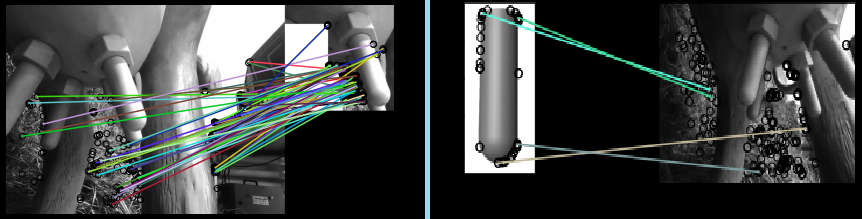
\includegraphics[width=0.9\textwidth]{images/cow_ransac.png}
%         \caption{RANSAC's behavior on the cow data set.}
%         \label{fig:ransac-results}
%     \end{figure}
    
% The following table 
% % \ref{tab:mav-results} displays 
% presents the results for the "MAV" algorithm. The optimizations presented are a combination of the offset and the averaging method.

% \begin{longtable}{|l|l||c|c|c|}                                              \hline
% \multicolumn{5}{|l|}{\textbf{MAV}}                                                       \\\hline
% \textbf{Offset}         & \textbf{Averaging Method}   
% & \textbf{Average Error}  & \textbf{Standard Deviation}  & \textbf{Execution Time}                 \\ \hline
% Fixed                   & Single Point                & 1.13            & 2.8              & 0.26 - 1.5 secs   \\ \hline
% Calculated              & Single Point                & 1.77            & 3.3              & 0.26 - 1.5 secs   \\ \hline
% Fixed                   & Average: 1/3rd              & \textbf{0.67}   & \textbf{2.4}     & 0.26 - 1.5 secs                     \\ \hline
% Calculated              & Average: 1/3rd              & 1.54            & 2.93             & 0.26 - 1.5 secs    \\ \hline
% Fixed                   & Average: 1/10th             & 0.96            & 2.55             & 0.26 - 1.5 secs     \\ \hline
% Calculated              & Average: 1/10th             & 1.51            & 2.87             & 0.26 - 1.5 secs    \\ \hline
% \caption{Overview of the best MAV results for the respective offset-averaging mechanisms combinations.} \label{tab:mav-results}                          
% \end{longtable}

% \subsubsection{Research Question 2}

% The second research question tackles the evaluation of the pose estimation of cow teats.

% \subsubsection{Quality Ranking of Predictions}


\subsection{Deliverables}
The following deliverables will be handed in with this master thesis:
\begin{itemize}
    \item This work produced three types of exploration-capable agents: environment-focused, object-focused and mixed-focused.
    The environment-focused agent is able to explore twice as many leaf nodes as the non-explorative models (71 versus 35 average leaf nodes per episode). This means that the average performance of the explorative agent explores 88\% of the small environment. 
    
    \item  The object-focused agent is able to scan at least 2 objects per episode on average. This translates to a scanning speed of 2500 time steps per object.
    
    \item Finally, the mixed exploration agent is able to keep up with the 2 objects per episode performance and explore an average 41 leaf nodes per episode, which covers 51\% of the environment, outperforming the 43\% coverage of object-focused models.
   
   \item A set of baselines are also handed in, used to analyze the performance of traditional methods for exploration (random actions, shortest path) and other state-of-the-art-inspired methods (object detection maximization, semantic curiosity, semantic entropy).
   
    \item The trained models for our proposed method in ONNX formats, including all other variants for voxel and octree exploration and an out-of-the-box Unity-ready reinforcement learning environment capable of reproducing the experiments and results.

    \item For future research, a set of Unity scenes that demonstrate the versatility of the reinforcement learning agent. These scenes further allow the creation of future benchmarks for other synthetic data models and use cases, which are not limited to machine learning approaches.
\end{itemize}



